\documentclass{article}

\usepackage{graphicx}
\usepackage[utf8]{inputenc}
\usepackage[T1]{fontenc}
\usepackage[francais]{babel}
\usepackage{hyperref}
\usepackage{amsmath,amsfonts,amssymb}
\usepackage{Tkz-Tab}
\usepackage{wrapfig}
\usepackage{verbatim}
\usepackage{array}

\begin{document}

\title{Gestion de flux dans le réseau
	\smallbreak
	TD n\degre5
	\smallbreak
	Modélisation mathématique
	\smallbreak
	Q4}
\author{Sibylle Roux \and Juliette Arazo \and Nicolas Le Gallo \and Tanguy Thomas}

\maketitle

\newpage

\tableofcontents

\newpage

\section{Essaies randoms}

\subsection{Loi Hypergeometrique}

\subsection{Preuve mathématique}
\begin{align}
\intertext{Paramètres}
N=20 ; n=3 ; m = 2 : P = \frac{2}{20}
\\
P(X=0)=\frac{
\begin{pmatrix}
m \\ 0
\end{pmatrix}
\times 
\begin{pmatrix}
N - m \\ 3
\end{pmatrix}
}{
\begin{pmatrix}
N \\ n
\end{pmatrix}
} 
\end{align}
\begin{align}
P(X=0)=\frac{
\begin{pmatrix}
2 \\ 0
\end{pmatrix}
\times 
\begin{pmatrix}
18 \\ 3
\end{pmatrix}
}{
\begin{pmatrix}
20 \\ 3
\end{pmatrix}
}= \frac{\frac{18\times17\times16}{3\times2\times1}}{\frac{20\times19\times18}{3 \times 2}} = 0.7158
\end{align} 
\begin{align}
P(X=1)=\frac{
\begin{pmatrix}
2 \\ 1
\end{pmatrix}
\times 
\begin{pmatrix}
18 \\ 2
\end{pmatrix}
}{
\begin{pmatrix}
20 \\ 3
\end{pmatrix}
}= \frac{2 \times \frac{18\times17}{2}}{\frac{20\times19\times18}{3 \times 2}} = 0.2684
\end{align}
\begin{align}
P(X=2)=\frac{
\begin{pmatrix}
2 \\ 2
\end{pmatrix}
\times 
\begin{pmatrix}
18 \\ 1
\end{pmatrix}
}{
\begin{pmatrix}
20 \\ 3
\end{pmatrix}
}= \frac{1 \times 18}{\frac{20\times19\times18}{3 \times 2}} = 0.0158
\end{align}

\begin{verbatim}
clear
clc
function s=hypergeo(N,n,P)
    M=P*N;
    s=0;
    for i=0:n-1
        if rand()<P
            M=M-1;
            N=N-1;
            s=s+1;
            P=M/N;
        else
            N=N-1;
            P=M/N;
        end         
    end
endfunction
N=20; n=3; P=2/20;t=[]; nb=10000
for j=1:nb+1
    t(j)=hypergeo(N,n,P); //100 tirages de loi hypergeo
end
frequences=tabul(t)// on calcule les frequences obtenues
frequences(:,2)=frequences(:,2)/nb
disp(frequences)
\end{verbatim}

\paragraph{Resultats d'un essai}
\begin{center}
\begin{tabular}{cccc}
nombre de succès & 0 & 1 & 2 \\
\hline
resultats programme & 0.0172 & 0.2728 & 0.7101 \\
\hline
resultats mathématiques & 0.0158 & 0.2684 & 0.7158 \\
\hline
\end{tabular}
\end{center}
Les valeurs obtenues par le programme sont proches des valeurs mathématiques. On peut en conclure que le programme retranscrit bien une loi hypergéométrique.

\section{Etude mathématique de la loi tente}

\subsection{Densité}

\subsubsection{Fonction}

$$
f(x)=\left\{
	\begin{array}{ll}
		1-|x| & \mbox{si} -1<=x<=1\\
		0 & \mbox{sinon}
	\end{array}
\right.
$$

\subsubsection{Représentation graphique}
\begin{center}
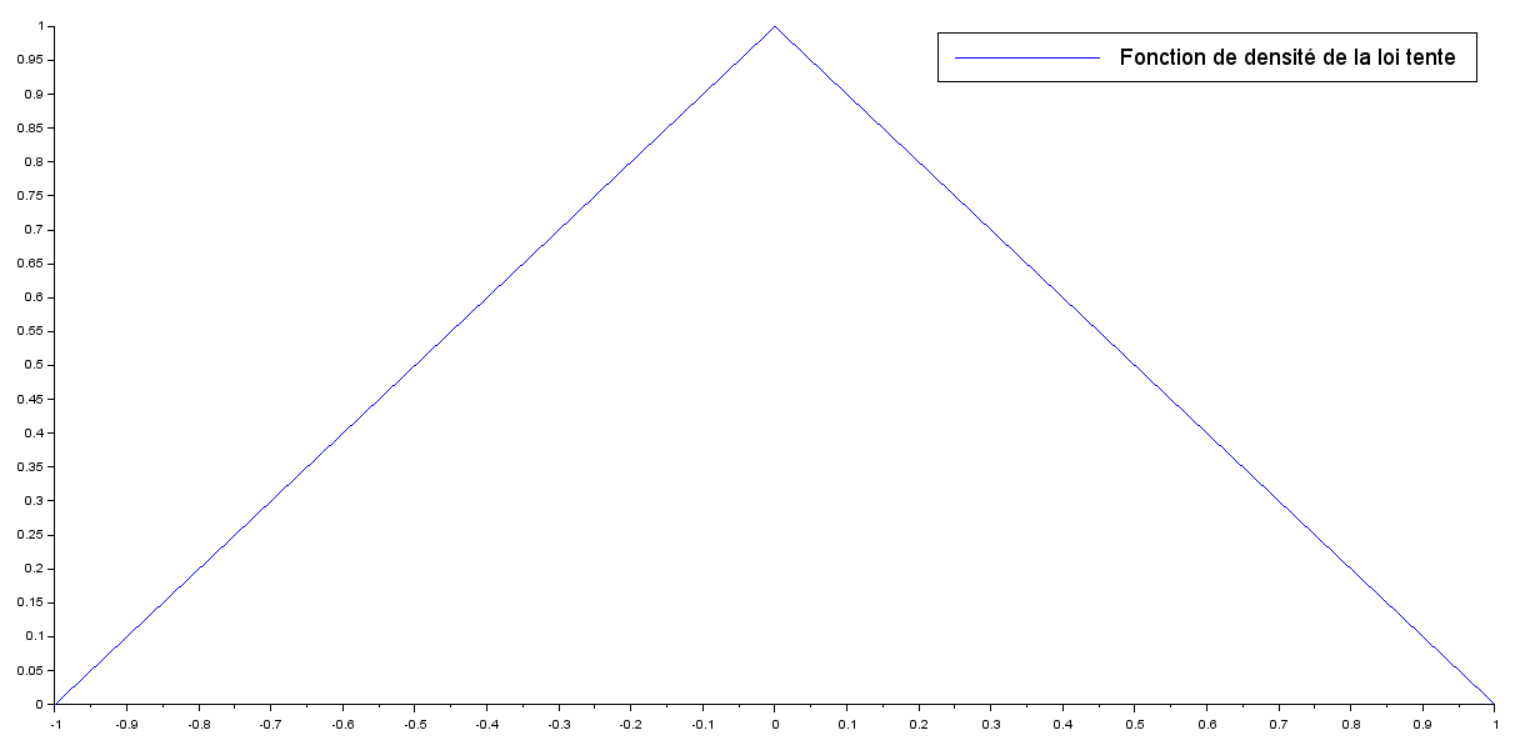
\includegraphics[width=425px]{img/tente.png}
\end{center}
\paragraph{}

\newpage

\subsection{Fonction de répartition}

\subsubsection{Fonction}

\begin{align}
f(x)=\left\{
	\begin{array}{llll}
		f(x)=0 &\mbox{pour } x<-1\\
		f(x)=1+x & \mbox{pour } -1<x<0 \\
		f(x)=1-x & \mbox{pour } 0<x<1 \\
		f(x)=0 & \mbox{pour } x>1 \\
	\end{array}
\right. 
\end{align}
\begin{align}
<=>
F(x)=\left\{
	\begin{array}{llll}
		\displaystyle \int_{- \infty }^{x} 0 \, \mathrm{d}x &\mbox{pour } x<-1\\
		\displaystyle \int_{- \infty }^{-1} 0 \, \mathrm{d}x+\displaystyle \int_{-1 }^{x} 1+x \, \mathrm{d}x &\mbox{pour } -1<x<0\\
		\displaystyle \int_{- \infty }^{-1} 0 \, \mathrm{d}x+\displaystyle \int_{-1 }^{0} 1+x \, \mathrm{d}x + \displaystyle \int_{0}^{x} 1-x \, \mathrm{d}x &\mbox{pour } 0<x<1\\
		\displaystyle \int_{- \infty }^{-1} 0 \, \mathrm{d}x+\displaystyle \int_{-1 }^{0} 1+x \, \mathrm{d}x + \displaystyle \int_{0}^{1} 1-x \, \mathrm{d}x+\displaystyle \int_{1}^{x} 0 \, \mathrm{d}x &\mbox{pour } x>1\\
	\end{array}
\right. 
\end{align}
\begin{align}
<=>
F(x)=\left\{
	\begin{array}{llll}
		0 &\mbox{pour } x<-1\\
		0 + \displaystyle \int_{-1 }^{x} 1+x \, \mathrm{d}x &\mbox{pour } -1<x<0\\
		0+\frac{1}{2}+\displaystyle \int_{0}^{x} 1-x \, \mathrm{d}x &\mbox{pour } 0<x<1\\
		0+\frac{1}{2}+\frac{1}{2}+\displaystyle \int_{1}^{x} 0 \, \mathrm{d}x &\mbox{pour } x>1\\
	\end{array}
\right. 
\end{align}
\begin{align}
<=>
F(x)=\left\{
	\begin{array}{llll}
		0 &\mbox{pour } x<-1\\
		\displaystyle \int_{-1 }^{x} 1+x \, \mathrm{d}x &\mbox{pour } -1<x<0\\
		\frac{1}{2}+\displaystyle \int_{0}^{x} 1-x \, \mathrm{d}x &\mbox{pour } 0<x<1\\
		1 &\mbox{pour } x>1\\
	\end{array}
\right. 
\end{align}
\begin{align}
<=>
F(x)=\left\{
	\begin{array}{llll}
		0 & \mbox{pour } x<-1\\
		\frac{1}{2} + x + \frac{x^2}{2} &\mbox{pour } -1<x<0\\
		\frac{1}{2} + x - \frac{x^2}{2} &\mbox{pour } 0<x<1\\
		1 & \mbox{pour } x>1\\
	\end{array}
\right.
\end{align}
\begin{align}
<=>
F(x)=\left\{
	\begin{array}{llll}
		0 & \mbox{pour } x<-1\\
		\frac{1}{2} \times (1 + 2x + x^2) &\mbox{pour } -1<x<0\\
		-\frac{1}{2} \times (-1 - 2x + x^2 +1 -1) &\mbox{pour } 0<x<1\\
		1 & \mbox{pour } x>1\\
	\end{array}
\right.
\end{align}
\begin{align}
<=>
F(x)=\left\{
	\begin{array}{llll}
		0 & \mbox{pour } x<-1\\
		\frac{(1+x)^2}{2} &\mbox{pour } -1<x<0\\
		\frac{2-(1-x)^2}{2} &\mbox{pour } 0<x<1\\
		1 & \mbox{pour } x>1\\
	\end{array}
\right.
\end{align}

\subsubsection{Représentation graphique}
\begin{center}
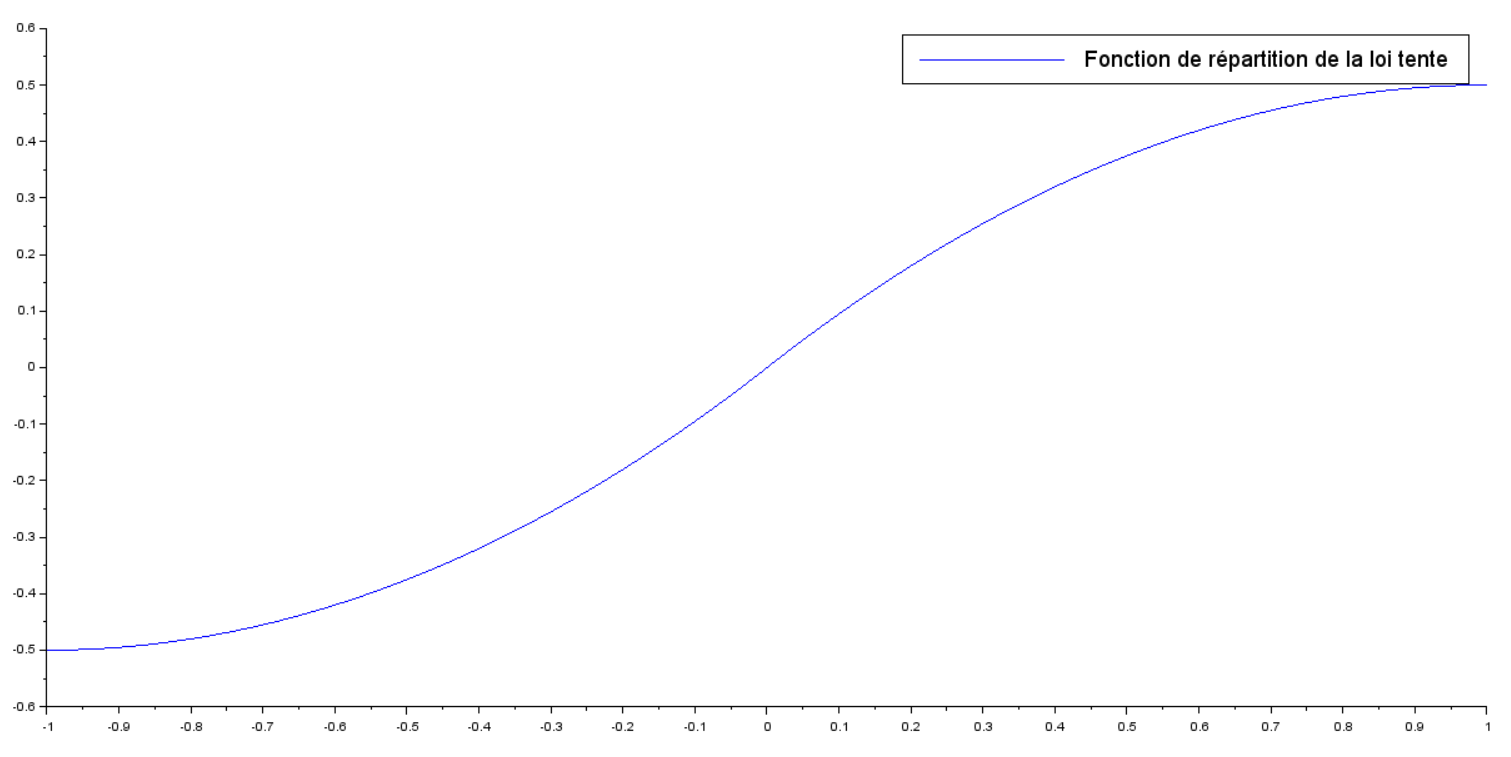
\includegraphics[width=425px]{img/tente_repartition.png}
\end{center}
\paragraph{}

\subsection{Inverse}

\subsubsection{Fonction}
\paragraph{} On va donc inverser les deux fonctions de répartitions de la loi tente% \eqref{tente}

\begin{align}
\left\{
	\begin{array}{ll}
		y_1=\frac{(1+x)^2}{2} &\mbox{pour } -1<x<0\\
		y_2=\frac{2-(1-x)^2}{2} &\mbox{pour } 0<x<1\\
	\end{array}
\right.
%\label{tente}
\end{align}
\begin{align}
y_1 & =\frac{(1+x)^2}{2} & y_2 & = \frac{2-(1-x)^2}{2} \\
2y_1 & = (1+x)^2 & 2y_2 & = 2 - (1-x)^2 \\
\sqrt{2y_1} & = 1+x & 2-2y_2 & = (1-x)^2 \\
x & = \sqrt{2y_1} - 1 & x & = 1- \sqrt{ 2-2y_2}
\end{align}
\begin{align}
\intertext{Donc la fonction inverse est :}
F^{-1}(x)=\left\{
		\begin{array}{ll}
			\sqrt{2x}-1 & \mbox{pour} 0<x<\frac{1}{2} \\
			1-\sqrt{2-2x} & \mbox{pour} \frac{1}{2}<x<1
		\end{array}
\right.
\end{align}


\subsubsection{Représentation graphique}
\begin{center}
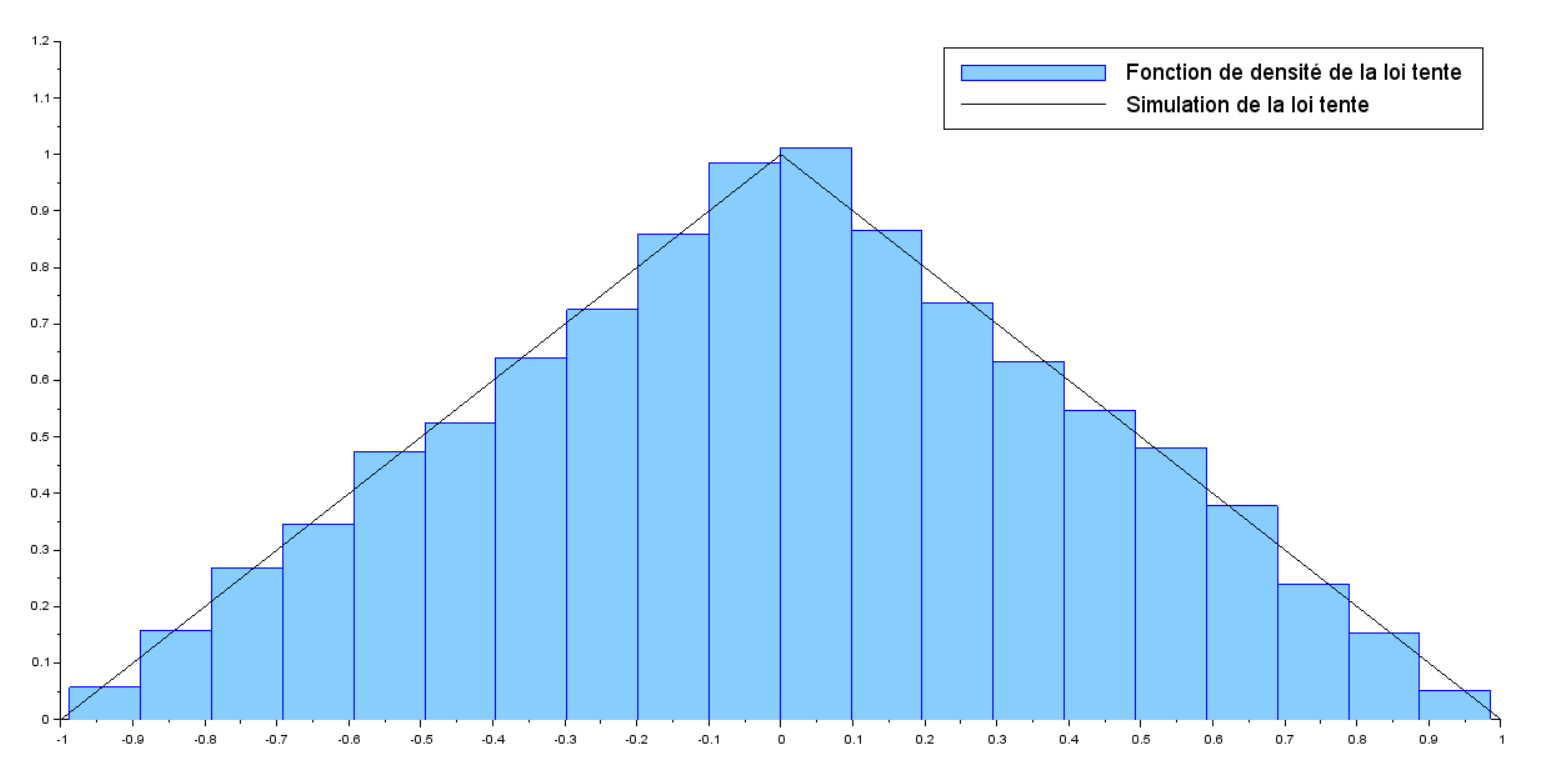
\includegraphics[width=425px]{img/tente_inversion.png}
\end{center}

\section{Inverse de la fonction de répartition de la loi exponentielle}

\subsection{Fonction}
\begin{align}
y & = 1 - e^{- \lambda t} \\
e^{- \lambda t} & =1-y \\
-\lambda t &= ln(1-y) \\
t &= - \frac{ln(1-y)}{\lambda}
\intertext{Donc la fonction inverse est : }
F^{-1}(t)&=- \frac{ln(1-y)}{\lambda}
\end{align}
\subsection{Représentation graphique}

\begin{center}
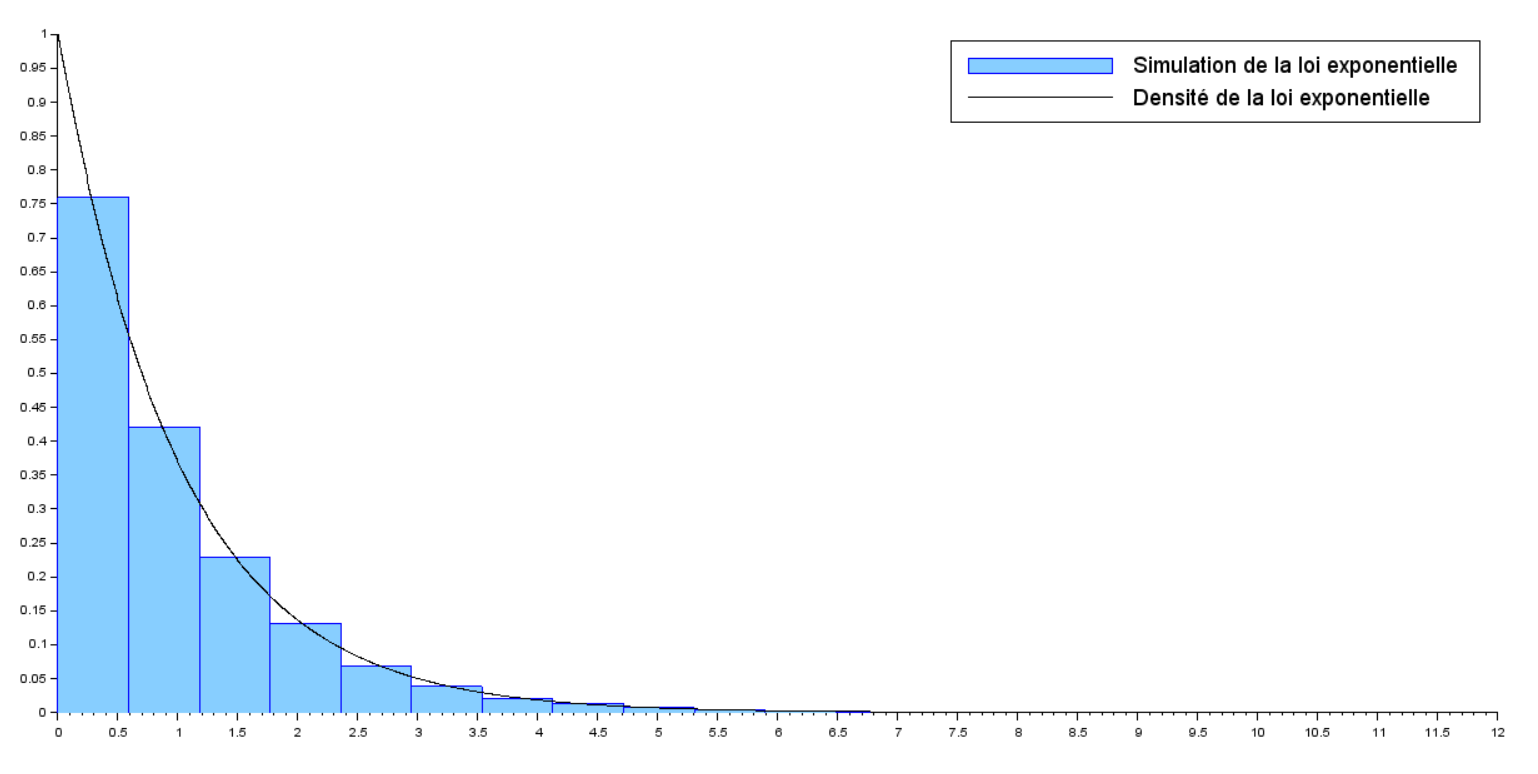
\includegraphics[width=425px]{img/inv_expo.png}
\end{center}
\paragraph{}

\section{Mesure de l'écart}



\section{Conclusion}
\paragraph{}

\newpage
\appendix

\section{Etude mathématique de la loi tente}
\subsection{Représentation graphique de la densité}
\begin{verbatim}
t = linspace(-1, 1, 301);
T = t;
i1 = (t>=-1) & (t<=1);
i2 = t>1 & t<-1;
T(i1)=1-abs(T(i1));
T(i2)=0
plot2d(t,T,style=2)
legend("Fonction de densité de la loi tente")
\end{verbatim}

\subsection{Représentation graphique de la fonction de répartition}
\begin{verbatim}
t = linspace(-1, 1, 301);
R=t;
i1 = t<-1;
i2 = (t>=-1) & (t<=0);
i3 = (t>0) & (t<=1);
i4 = t>1;
R(i1) = 0;
R(i2) = 0.5 + R(i2)+((R(i2)^2)/2)
R(i3) = 0.5 + R(i3)-((R(i3)^2)/2)
R(i4) = 1;
plot2d(t,R,style=2)
legend("Fonction de répartition de la loi tente")
\end{verbatim}

\subsection{Représentation graphique de la fonction inverse}
\begin{verbatim}
function t = tente(n)
    u = rand(n, 1);
    t = u
    i1 = u < 1/2
    i2 = u >= 1/2
    t(i1) = sqrt(2*t(i1))-1;
    t(i2) = 1-sqrt(2-2*t(i2));
endfunction
histplot(20,tente(10000))

// Fonction de densité 

t = linspace(-1, 1, 301);
T = t;
i1 = (t>=-1) & (t<=1);
i2 = t>1 & t<-1;
T(i1)=1-abs(T(i1));
T(i2)=0
plot2d(t,T,style=1)

legend("Fonction de densité de la loi tente","Simulation de la loi tente")
\end{verbatim}

\section{Inverse de la fonction de répartition}

\subsection{Représentation graphique de la fonction inverse}
\begin{verbatim}
function t = expo(l,n)
    u = rand(n, 1);
    t = u
    t = -log(1-t)/l 
endfunction
histplot(20,expo(1,100000))

// Fonction de densité de la loi exponentielle

a=0:0.01:12;
lambda=1;
b=lambda*exp(-lambda*a);
plot2d2(a,b,style=1)

legend("Simulation de la loi exponentielle","Densité de la loi exponentielle")
\end{verbatim}

%----------------------------------


\end{document}